\documentclass[9pt]{beamer}

% Beamer style
%\usetheme[secheader]{Madrid}
% \usetheme{CambridgeUS}
\useoutertheme{infolines}
\usecolortheme[rgb={0.65,0.15,0.25}]{structure}
% \usefonttheme[onlymath]{serif}
\beamertemplatenavigationsymbolsempty
%\AtBeginSubsection

% Packages
%\usepackage[french]{babel}
\usepackage[latin1]{inputenc}
\usepackage{color}
\usepackage{xspace}
\usepackage{dsfont, stmaryrd}
\usepackage{amsmath, amsfonts, amssymb, stmaryrd}
\usepackage{epsfig}
\usepackage{tikz}
\usepackage{url}
% \usepackage{ulem}
\usepackage{/home/robin/LATEX/Biblio/astats}
%\usepackage[all]{xy}
\usepackage{graphicx}
\usepackage{enumerate}
\usepackage{xspace}

% Maths
% \newtheorem{theorem}{Theorem}
% \newtheorem{definition}{Definition}
\newtheorem{proposition}{Proposition}
% \newtheorem{assumption}{Assumption}
% \newtheorem{algorithm}{Algorithm}
% \newtheorem{lemma}{Lemma}
% \newtheorem{remark}{Remark}
% \newtheorem{exercise}{Exercise}
% \newcommand{\propname}{Prop.}
% \newcommand{\proof}{\noindent{\sl Proof:}\quad}
% \newcommand{\eproof}{$\blacksquare$}

% \setcounter{secnumdepth}{3}
% \setcounter{tocdepth}{3}
\newcommand{\pref}[1]{\ref{#1} p.\pageref{#1}}
\newcommand{\qref}[1]{\eqref{#1} p.\pageref{#1}}

% Colors : http://latexcolor.com/
\definecolor{darkred}{rgb}{0.65,0.15,0.25}
\definecolor{darkgreen}{rgb}{0,0.4,0}
\definecolor{darkred}{rgb}{0.65,0.15,0.25}
\definecolor{amethyst}{rgb}{0.6, 0.4, 0.8}
\definecolor{asparagus}{rgb}{0.53, 0.66, 0.42}
\definecolor{applegreen}{rgb}{0.55, 0.71, 0.0}
\definecolor{awesome}{rgb}{1.0, 0.13, 0.32}
\definecolor{blue-green}{rgb}{0.0, 0.87, 0.87}
\definecolor{red-ggplot}{rgb}{0.52, 0.25, 0.23}
\definecolor{green-ggplot}{rgb}{0.42, 0.58, 0.00}
\definecolor{purple-ggplot}{rgb}{0.34, 0.21, 0.44}
\definecolor{blue-ggplot}{rgb}{0.00, 0.49, 0.51}

% Commands
\newcommand{\backupbegin}{
   \newcounter{finalframe}
   \setcounter{finalframe}{\value{framenumber}}
}
\newcommand{\backupend}{
   \setcounter{framenumber}{\value{finalframe}}
}
\newcommand{\emphase}[1]{\textcolor{darkred}{#1}}
\newcommand{\comment}[1]{\textcolor{gray}{#1}}
\newcommand{\paragraph}[1]{\textcolor{darkred}{#1}}
\newcommand{\refer}[1]{{\small{\textcolor{gray}{{\cite{#1}}}}}}
\newcommand{\Refer}[1]{{\small{\textcolor{gray}{{[#1]}}}}}
\newcommand{\goto}[1]{{\small{\textcolor{blue}{[\#\ref{#1}]}}}}
\renewcommand{\newblock}{}

\newcommand{\tabequation}[1]{{\medskip \centerline{#1} \medskip}}
% \renewcommand{\binom}[2]{{\left(\begin{array}{c} #1 \\ #2 \end{array}\right)}}

% Variables 
\newcommand{\Abf}{{\bf A}}
\newcommand{\Beta}{\text{B}}
\newcommand{\Bcal}{\mathcal{B}}
\newcommand{\Bias}{\xspace\mathbb B}
\newcommand{\Cor}{{\mathbb C}\text{or}}
\newcommand{\Cov}{{\mathbb C}\text{ov}}
\newcommand{\cl}{\text{\it c}\ell}
\newcommand{\Ccal}{\mathcal{C}}
\newcommand{\cst}{\text{cst}}
\newcommand{\Dcal}{\mathcal{D}}
\newcommand{\Ecal}{\mathcal{E}}
\newcommand{\Esp}{\xspace\mathbb E}
\newcommand{\Espt}{\widetilde{\Esp}}
\newcommand{\Covt}{\widetilde{\Cov}}
\newcommand{\Ibb}{\mathbb I}
\newcommand{\Fcal}{\mathcal{F}}
\newcommand{\Gcal}{\mathcal{G}}
\newcommand{\Gam}{\mathcal{G}\text{am}}
\newcommand{\Hcal}{\mathcal{H}}
\newcommand{\Jcal}{\mathcal{J}}
\newcommand{\Lcal}{\mathcal{L}}
\newcommand{\Mt}{\widetilde{M}}
\newcommand{\mt}{\widetilde{m}}
\newcommand{\Nbb}{\mathbb{N}}
\newcommand{\Mcal}{\mathcal{M}}
\newcommand{\Ncal}{\mathcal{N}}
\newcommand{\Ocal}{\mathcal{O}}
\newcommand{\pt}{\widetilde{p}}
\newcommand{\Pt}{\widetilde{P}}
\newcommand{\Pbb}{\mathbb{P}}
\newcommand{\Pcal}{\mathcal{P}}
\newcommand{\Qcal}{\mathcal{Q}}
\newcommand{\qt}{\widetilde{q}}
\newcommand{\Rbb}{\mathbb{R}}
\newcommand{\Sbb}{\mathbb{S}}
\newcommand{\Scal}{\mathcal{S}}
\newcommand{\st}{\widetilde{s}}
\newcommand{\St}{\widetilde{S}}
\newcommand{\Tcal}{\mathcal{T}}
\newcommand{\todo}{\textcolor{red}{TO DO}}
\newcommand{\Ucal}{\mathcal{U}}
\newcommand{\Un}{\math{1}}
\newcommand{\Vcal}{\mathcal{V}}
\newcommand{\Var}{\mathbb V}
\newcommand{\Vart}{\widetilde{\Var}}
\newcommand{\Zcal}{\mathcal{Z}}

% Symboles & notations
\newcommand\independent{\protect\mathpalette{\protect\independenT}{\perp}}\def\independenT#1#2{\mathrel{\rlap{$#1#2$}\mkern2mu{#1#2}}} 
\renewcommand{\d}{\text{\xspace d}}
\newcommand{\gv}{\mid}
\newcommand{\ggv}{\, \| \, }
% \newcommand{\diag}{\text{diag}}
\newcommand{\card}[1]{\text{card}\left(#1\right)}
\newcommand{\trace}[1]{\text{tr}\left(#1\right)}
\newcommand{\matr}[1]{\boldsymbol{#1}}
\newcommand{\matrbf}[1]{\mathbf{#1}}
\newcommand{\vect}[1]{\matr{#1}} %% un peu inutile
\newcommand{\vectbf}[1]{\matrbf{#1}} %% un peu inutile
\newcommand{\trans}{\intercal}
\newcommand{\transpose}[1]{\matr{#1}^\trans}
\newcommand{\crossprod}[2]{\transpose{#1} \matr{#2}}
\newcommand{\tcrossprod}[2]{\matr{#1} \transpose{#2}}
\newcommand{\matprod}[2]{\matr{#1} \matr{#2}}
\DeclareMathOperator*{\argmin}{arg\,min}
\DeclareMathOperator*{\argmax}{arg\,max}
\DeclareMathOperator{\sign}{sign}
\DeclareMathOperator{\tr}{tr}
\newcommand{\ra}{\emphase{$\rightarrow$} \xspace}

% Hadamard, Kronecker and vec operators
\DeclareMathOperator{\Diag}{Diag} % matrix diagonal
\DeclareMathOperator{\diag}{diag} % vector diagonal
\DeclareMathOperator{\mtov}{vec} % matrix to vector
\newcommand{\kro}{\otimes} % Kronecker product
\newcommand{\had}{\odot}   % Hadamard product

% TikZ
\newcommand{\nodesize}{2em}
\newcommand{\edgeunit}{2.5*\nodesize}
\newcommand{\edgewidth}{1pt}
\tikzstyle{node}=[draw, circle, fill=black, minimum width=.75\nodesize, inner sep=0]
\tikzstyle{square}=[rectangle, draw]
\tikzstyle{param}=[draw, rectangle, fill=gray!50, minimum width=\nodesize, minimum height=\nodesize, inner sep=0]
\tikzstyle{hidden}=[draw, circle, fill=gray!50, minimum width=\nodesize, inner sep=0]
\tikzstyle{hiddenred}=[draw, circle, color=red, fill=gray!50, minimum width=\nodesize, inner sep=0]
\tikzstyle{observed}=[draw, circle, minimum width=\nodesize, inner sep=0]
\tikzstyle{observedred}=[draw, circle, minimum width=\nodesize, color=red, inner sep=0]
\tikzstyle{eliminated}=[draw, circle, minimum width=\nodesize, color=gray!50, inner sep=0]
\tikzstyle{empty}=[draw, circle, minimum width=\nodesize, color=white, inner sep=0]
\tikzstyle{blank}=[color=white]
\tikzstyle{nocircle}=[minimum width=\nodesize, inner sep=0]

\tikzstyle{edge}=[-, line width=\edgewidth]
\tikzstyle{edgebendleft}=[-, >=latex, line width=\edgewidth, bend left]
\tikzstyle{edgebendright}=[-, >=latex, line width=\edgewidth, bend right]
\tikzstyle{lightedge}=[-, line width=\edgewidth, color=gray!50]
\tikzstyle{lightedgebendleft}=[-, >=latex, line width=\edgewidth, bend left, color=gray!50]
\tikzstyle{lightedgebendright}=[-, >=latex, line width=\edgewidth, bend right, color=gray!50]
\tikzstyle{edgered}=[-, line width=\edgewidth, color=red]
\tikzstyle{edgebendleftred}=[-, >=latex, line width=\edgewidth, bend left, color=red]
\tikzstyle{edgebendrightred}=[-, >=latex, line width=\edgewidth, bend right, color=red]

\tikzstyle{arrow}=[->, >=latex, line width=\edgewidth]
\tikzstyle{arrowbendleft}=[->, >=latex, line width=\edgewidth, bend left]
\tikzstyle{arrowbendright}=[->, >=latex, line width=\edgewidth, bend right]
\tikzstyle{arrowred}=[->, >=latex, line width=\edgewidth, color=red]
\tikzstyle{arrowbendleftred}=[->, >=latex, line width=\edgewidth, bend left, color=red]
\tikzstyle{arrowbendrightred}=[->, >=latex, line width=\edgewidth, bend right, color=red]
\tikzstyle{arrowblue}=[->, >=latex, line width=\edgewidth, color=blue]
\tikzstyle{dashedarrow}=[->, >=latex, dashed, line width=\edgewidth]
\tikzstyle{dashededge}=[-, >=latex, dashed, line width=\edgewidth]
\tikzstyle{dashededgebendleft}=[-, >=latex, dashed, line width=\edgewidth, bend left]
\tikzstyle{lightarrow}=[->, >=latex, line width=\edgewidth, color=gray!50]

\renewcommand{\chaptername}{Lecture}

\newcommand{\fignet}{/home/robin/RECHERCHE/RESEAUX/EXPOSES/FIGURES}
\newcommand{\figeco}{/home/robin/RECHERCHE/ECOLOGIE/EXPOSES/FIGURES}
\newcommand{\figCMR}{/home/robin/Bureau/RECHERCHE/ECOLOGIE/CountPCA/sparsepca/Article/Network_JCGS/trunk/figs}
\newcommand{\figeconet}{/home/robin/Bureau/RECHERCHE/ECOLOGIE/EXPOSES/1904-EcoNet-Lyon/Figs}
\newcommand{\figbarents}{/home/robin/Bureau/CountPCA/sparsepca/Pgm/PLNnetwork/barent_fish/output_barents}
\newcommand{\figbordeaux}{/home/robin/Bureau/RECHERCHE/EXPOSES/RESEAUX/1904-Bordeaux}

%==================================================================%==================================================================
\begin{document}
%==================================================================
%==================================================================
\title{Some statistical models for ecological networks: \\
  Network topology}
\author{S. Robin}
\date{\today}
\maketitle

\frame{\frametitle{Outline} \tableofcontents}

%==================================================================%==================================================================
\section{Introduction} 
% \frame{\frametitle{Outline} \tableofcontents[currentsection]}
%==================================================================
\frame{\frametitle{Different types of networks}

  \paragraph{Network =} natural and convenient way to represent ecological 'interactions' \refer{Bas09}

  \bigskip \bigskip \pause
  \paragraph{Many types of networks:} trophic, plant-pollinator, 'interaction'

  \bigskip \bigskip \pause
  \paragraph{Aim:} understand their organisations, i.e. analyse their {\sl topology}
  \begin{overprint}
    \onslide<4>
    \begin{tabular}{p{.35\textwidth}p{.55\textwidth}}
      \begin{tabular}{p{.35\textwidth}}
        Do trophic levels actually exist? \\
        \\
        {\tiny \url{en.wikipedia.org/wiki/Trophic_coherence}}
      \end{tabular}
      &
      \begin{tabular}{p{.55\textwidth}}
        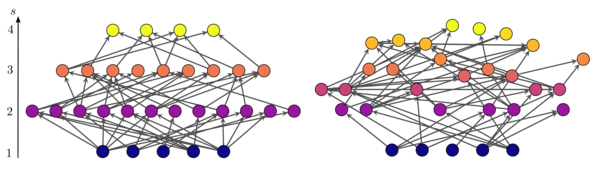
\includegraphics[trim=20 0 300 0, width=.35\textwidth, clip]{\figeco/WikipediaTrophicNetwork} \\
        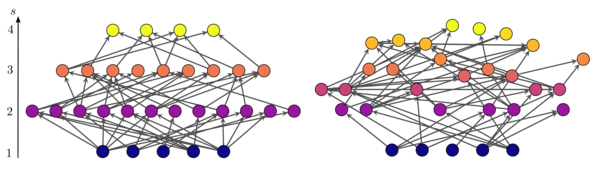
\includegraphics[trim=310 0 0 0, width=.35\textwidth, clip]{\figeco/WikipediaTrophicNetwork} 
      \end{tabular} 
    \end{tabular}
    \onslide<5>
    \begin{tabular}{p{.35\textwidth}p{.55\textwidth}}
      \begin{tabular}{p{.35\textwidth}}
        Generalist vs specialist pollinators?  \\
        \\
        {\tiny \url{seibutsu.biology.kyushu-u.ac.jp/~satake}}
      \end{tabular}
      &
      \begin{tabular}{p{.55\textwidth}}
        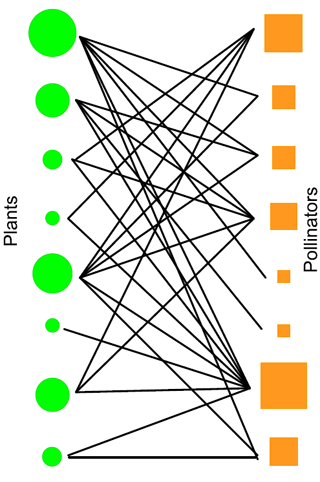
\includegraphics[height=.45\textwidth,angle=270]{\figeco/SatakePlantPollinatorNetwork}
      \end{tabular} 
    \end{tabular}
    \onslide<6>
    \begin{tabular}{p{.35\textwidth}p{.55\textwidth}}
      \begin{tabular}{p{.35\textwidth}}
        Is the network 'organized'? \\
        \\
        If so, how? \\
        \\
        {\tiny \url{www.allisonbarner.com}}
      \end{tabular}
      &
      \begin{tabular}{p{.55\textwidth}}
        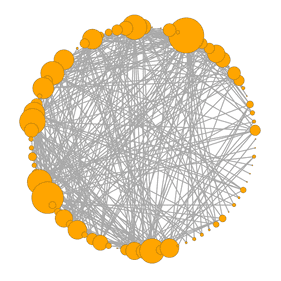
\includegraphics[width=.4\textwidth]{\figeco/BarnerEcologicalNetwork}
      \end{tabular} 
    \end{tabular}
  \end{overprint}
}
  
%==================================================================
\frame{\frametitle{Modelling approach}

  \paragraph{Mathematical counterpart:} 
  $$
  \text{ecological {\sl network}}
  \quad \leftrightarrow \quad
  \text{random {\sl graph}}  
  $$

  \bigskip \pause
  \paragraph{Random graph:}   $n$ nodes  = species, individuals, ... ($1 \leq i, j \leq n$), 
  $$
  Y_{ij} = \text{ 'value' of the edge between node $i$ and $j$}
  $$
  Random graph model = joint distribution of all edge values:
  $$
  p(\{Y_{ij}\}_{i, j})
  \qquad \rightarrow \qquad \simeq n^2 \text{ random variables}
  $$

  \bigskip \bigskip \pause
  \begin{tabular}{p{.35\textwidth}p{.6\textwidth}}
    \paragraph{Type of network:} & \paragraph{Type of edge:} \\ %~ \\
      directed / undirected & $Y_{ij} = Y_{ji}$ or not \\ %~ \\
      binary / valued ('weighted') & $Y_{ij} \in \{0, 1\}$ or $\Rbb$ \\ %~ \\
      multivariate ('multiplex') & $Y_{ij} \in \{0, 1\}^d$ or $\Rbb^d$ \\
      & or $\{0, 1\} \times \{a, b, c, d\} \times \Nbb \times \Rbb$
  \end{tabular}

}

%==================================================================
\frame{\frametitle{A model: what for?}

  Many different aims: \\~
  \begin{enumerate}[($a$)]
    \item \emphase{Mechanistic} model: pretends to encode the process that actually generated the data \\~
    \item \emphase{Empirical} model: enables to simulate data similar to the observed ones \\~ 
    \item \emphase{Null} model: serves as a reference to detect 'unexpected behaviors' 
  \end{enumerate}

  \bigskip \bigskip \pause
  \paragraph{Here,} focus on 
  \begin{itemize}
    \item ($b$) and ($c$): empirical and null models
    \item for binary networks (with some extensions)
  \end{itemize}


}


\section{Some random graph models} 
\frame{\frametitle{Outline} \tableofcontents[currentsection]}
%******************************************************************************
\subsection{Degree-based models}

%******************************************************************************
\subsection{Latent-space models}

%******************************************************************************
\subsection{Accounting for covariates}


\section{Block-models} 
\frame{\frametitle{Outline} \tableofcontents[currentsection]}
\begin{itemize}
 \item \cite{LDV15}, \cite{MPD14}
\end{itemize}


%******************************************************************************
\subsection{Stochastic block-model (SBM)}

%******************************************************************************
\subsection{Latent block-model (LBM)}


\section{Network motifs} 
\frame{\frametitle{Outline} \tableofcontents[currentsection]}
%******************************************************************************
\subsection{A null model}

%******************************************************************************
\subsection{B-motifs}



\section{Discussion} 
\frame{\frametitle{Outline} \tableofcontents[currentsection]}
%==================================================================
\frame{\frametitle{All models are wrong ...}

  but some are useful
  
  \bigskip \bigskip \pause 
  \paragraph{Statistical models} can be useful
  \begin{itemize}
   \item to exhibit latent structure
   \item to correct for expected effects (e.g. covariates) and enhanced unexpected ones
   \item to serve as (not too) null model to be compared with observation (and to exhibit some {\sl residual} structure)
  \end{itemize}
  \ra Always tailored for a given purpose (no generic model)

  \bigskip \bigskip \pause
  \paragraph{'Null model'} sometimes refers to resampled-based null distribution:
  \begin{itemize}
   \item appealing because (reasonably) easy to implement
   \item appealing because no distribution assumption seems to be made
   \item confusing because underlying assumptions are not always explicit
  \end{itemize}
    

}


%==================================================================
\backupbegin

\frame[allowframebreaks]{ \frametitle{References} 
  {\tiny
   \bibliography{/home/robin/Biblio/BibGene}
   \bibliographystyle{alpha}
  }
}

% \section*{Backup} 
% %==================================================================
\frame{\frametitle{A series of indicators}

\begin{itemize}
 \item Density, connectivity, centrality, nestedness: \cite{BJM03}
 \item ... to be interpreted, most often in the framework of an (implicit) (population) dynamic model (e.g.Lotka-Volterra): \cite{ThF10}, \cite{GiB12}
 \item \cite{Bas09}, 
 \item Global: clusters
 \item Local: motifs
\end{itemize}
}

%==================================================================
\frame{ \frametitle{ERGMs}

}


\backupend

%==================================================================
%==================================================================
\end{document}
%==================================================================
%==================================================================

\begin{tabular}{p{.45\textwidth}p{.45\textwidth}}
  \begin{tabular}{p{.45\textwidth}}
  \end{tabular}
  &
  \begin{tabular}{p{.45\textwidth}}
  \end{tabular} 
\end{tabular}
